
\documentclass{beamer}
\usetheme{Darmstadt}
\usecolortheme{seahorse}
\usepackage[utf8]{inputenc}
\usefonttheme{professionalfonts}
\usepackage{tikz}
\usepackage{tabularx}
\usepackage{colortbl}
\usepackage{graphicx}
%\usepackage{epstopdf}

\usetikzlibrary{calc}
\pgfdeclarelayer{background}
\pgfdeclarelayer{foreground}
\pgfsetlayers{background,main,foreground}

\graphicspath{images/}

\let\oldfootnotesize\footnotesize
\renewcommand*{\footnotesize}{\oldfootnotesize\tiny}

\setbeamertemplate{note page}[plain]

\title{Software Development Processes}
\author{Maksym Borodin}

\begin{document}
\frame{\titlepage}
\frame{\frametitle{Table of contents}\tableofcontents}

\section{Introduction}
\begin{frame}
\frametitle{Introduction}
\begin{itemize}
    \item<1-> Five questions
    \item<2-> What? - software definition
    \item<3-> Why? - do we really need it?
    \item<4-> How? - Process
        \begin{itemize}
            \item<2-> \textbf{Roles} and \textbf{responsibilities}
            \item<3-> \textbf{Interaction} between subteams, with customers etc
            \item<4-> Production \textbf{environment}
            \item<5-> Required \textbf{artifacts}
            \note{Software production team is \textbf{heterogeneous} therefore \textbf{Artifacts} are required for better communication. They can be \textbf{skipped} in in scientific environment, nevertheless some of them are very \textbf{useful}}
        \end{itemize}
    \item<5-> Who? - Team
        \begin{itemize}
            \item<6-> Manager
            \item<7-> Architect
            \item<8-> Technical leader
            \item<9-> Dev team
            \item<10-> QA team
            \item<11-> Marketing team
            \item<12-> Other support teams
                \note{Other teams: system administrators, lawyers (licensing, customer relations, patents), in some caases - patent team}
        \end{itemize}
    \item<13-> When? - Product delivery plan
\end{itemize}
\end{frame}


\section{Product lifecycle}
\begin{frame}
\frametitle{Research life cycle}
\note[item]<2>{Artifacts can be omitted. Useful artifacts will be shown and explained}
\note[item]<2>{Artifacts - magnifying glass to see target product}
\note[item]<2>{Requirements artifact. Give example: too wide, to detailed, good}
\begin{figure}
    \resizebox{10.0cm}{!}{
        \includegraphics{images/rlc.png}
        %\input{images/rlc_opt}
    }
\end{figure}
\begin{center}
    \resizebox{10cm}{!}{
    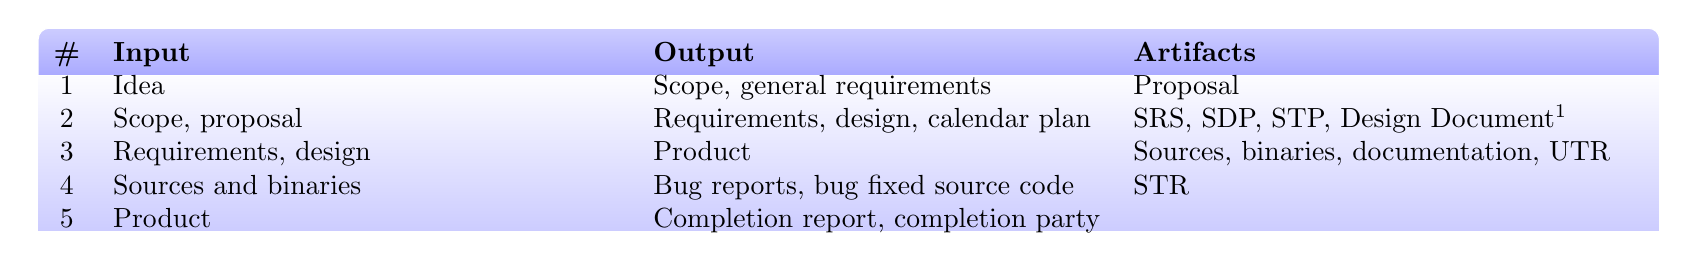
\begin{tikzpicture}
        \node (tbl) {
            \begin{tabularx}{1.7\textwidth}{cXlll}
                \arrayrulecolor{cyan}
                \textbf{\#} & \textbf{Input}& \textbf{Output} & \textbf{Artifacts} & \\
                1 & Idea & Scope, general requirements & Proposal \\
                2 & Scope, proposal & Requirements, design, calendar plan & SRS, SDP, STP, Design Document\footnotemark \\
                3 & Requirements, design & Product & Sources, binaries, documentation, UTR \\
                4 & Sources and binaries & Bug reports, bug fixed source code & STR \\
                5 & Product & Completion report, completion party
            \end{tabularx}
        };
        \begin{pgfonlayer}{background}
            \draw[rounded corners,top color=blue!20,bottom color=blue!40,draw=white] ($(tbl.north west)+(0.14,0)$)  rectangle ($(tbl.north east)-(0.13,0.9)$);
            %\draw[rounded corners,top color=white,bottom color=blue!40,middle color=white,draw=blue!20] ($(tbl.south west) +(0.13,0.2)$) rectangle ($(tbl.south east)-(0.12,0)$);
            \draw[top color=blue!1,bottom color=blue!20,draw=white] ($(tbl.north east)-(0.13,0.6)$) rectangle ($(tbl.south west)+(0.13,0.2)$);
        \end{pgfonlayer}
    \end{tikzpicture}}
\end{center}
\footnotetext[1]{\small Design document depends on chosen development process and could be SDD, HLD/DLD etc}
\end{frame}

\begin{frame}
\frametitle{Product life cycle}
\begin{figure}
    \resizebox{10.0cm}{!}{
        \includegraphics{images/rlc.png}
        %\input{images/rlc_opt}
    }
\end{figure}
\begin{center}
    \resizebox{10cm}{!}{
    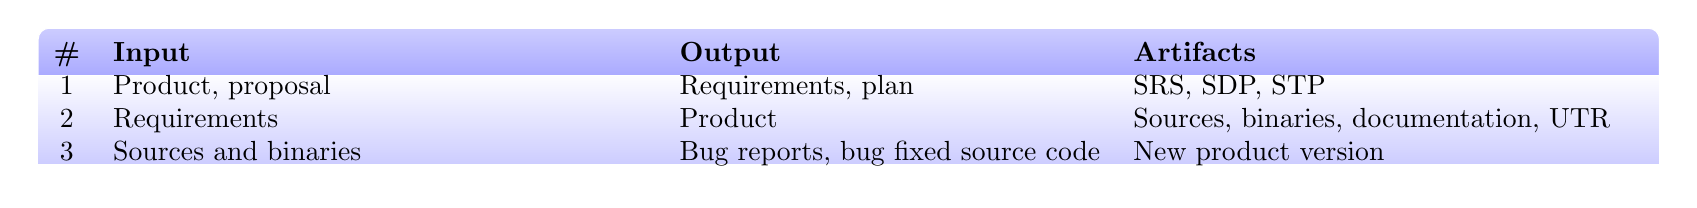
\begin{tikzpicture}
        \node (tbl) {
            \begin{tabularx}{1.7\textwidth}{cXlll}
                \arrayrulecolor{cyan}
                \textbf{\#} & \textbf{Input}& \textbf{Output} & \textbf{Artifacts} & \\
                1 & Product, proposal & Requirements, plan & SRS, SDP, STP \\
                2 & Requirements & Product & Sources, binaries, documentation, UTR \\
                3 & Sources and binaries & Bug reports, bug fixed source code & New product version
            \end{tabularx}
        };
        \begin{pgfonlayer}{background}
            \draw[rounded corners,top color=blue!20,bottom color=blue!40,draw=white] ($(tbl.north west)+(0.14,0)$)  rectangle ($(tbl.north east)-(0.13,0.9)$);
            %\draw[rounded corners,top color=white,bottom color=blue!40,middle color=white,draw=blue!20] ($(tbl.south west) +(0.13,0.2)$) rectangle ($(tbl.south east)-(0.12,0)$);
            \draw[top color=blue!1,bottom color=blue!20,draw=white] ($(tbl.north east)-(0.13,0.6)$) rectangle ($(tbl.south west)+(0.13,0.2)$);
        \end{pgfonlayer}
    \end{tikzpicture}}
\end{center}

\end{frame}

\begin{frame}
\frametitle{RLC and PLC comparison}
\resizebox{10cm}{!}{
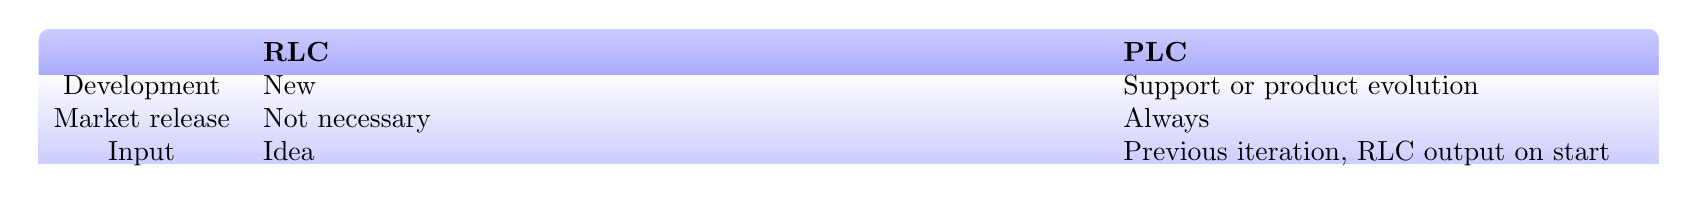
\begin{tikzpicture}
        \node (tbl) {
            \begin{tabularx}{1.7\textwidth}{cXlll}
                \arrayrulecolor{cyan}
                 \textbf{}& \textbf{RLC} & \textbf{PLC} & \\
                Development& New & Support or product evolution \\
                Market release & Not necessary & Always \\
                Input & Idea & Previous iteration, RLC output on start
            \end{tabularx}
        };
        \begin{pgfonlayer}{background}
            \draw[rounded corners,top color=blue!20,bottom color=blue!40,draw=white] ($(tbl.north west)+(0.14,0)$)  rectangle ($(tbl.north east)-(0.13,0.9)$);
            %\draw[rounded corners,top color=white,bottom color=blue!40,middle color=white,draw=blue!20] ($(tbl.south west) +(0.13,0.2)$) rectangle ($(tbl.south east)-(0.12,0)$);
            \draw[top color=blue!1,bottom color=blue!20,draw=white] ($(tbl.north east)-(0.13,0.6)$) rectangle ($(tbl.south west)+(0.13,0.2)$);
        \end{pgfonlayer}
\end{tikzpicture}}

\begin{itemize}
    \item<1-> RLC is a new product \textbf{development}
    \item<2-> PLC is product \textbf{support} and \textbf{ evolution}
    \item<3-> RLC is \textbf{not necessary releases} a product on market
    \item<4-> PLC \textbf{always} releases product on market
    \item<3-> PLC iteratively runs on top of previous input with initial input from RLC
\end{itemize}
\end{frame}


\section{Development process}
\begin{frame}
\frametitle{Waterfall}
\note{Is a model}
\end{frame}

\begin{frame}
\frametitle{Iterative}

\end{frame}

\begin{frame}
\frametitle{Agile}
\note{Is a methodology}

\end{frame}

\begin{frame}
\frametitle{SCRUM}
\begin{figure}
    \resizebox{10.0cm}{!}{
        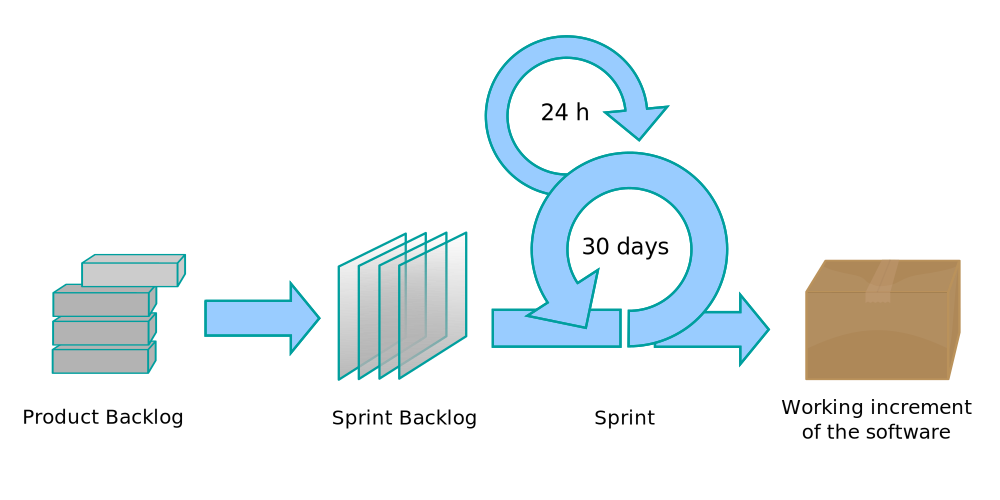
\includegraphics{images/Scrum_process.png}
    }
\end{figure}

\end{frame}

\begin{frame}
\frametitle{Test Driven Development}

\end{frame}

\begin{frame}
\frametitle{Behavior driven development}
\note{Say few fords on methodologies combination, i.e. SCRUM + TDD}
\end{frame}



\section{Development in HEP}
\begin{frame}
\frametitle{Scale view}
What?
Affects:
Possible answers
\end{frame}

\begin{frame}
\frametitle{Task view}
What?
Affects:
Possible answers
\end{frame}


\section{Tools}
\begin{frame}
\frametitle{Project management}

\end{frame}

\begin{frame}
\frametitle{Version control}

\end{frame}

\begin{frame}
\frametitle{Code review}

\end{frame}

\begin{frame}
\frametitle{Code verification}

\end{frame}

\begin{frame}
\frametitle{Continuous integration}

\end{frame}


\section{Useful methodics}
\begin{frame}
\frametitle{Test Driven Development}

\end{frame}

\begin{frame}
\frametitle{Behavior driven development}

\end{frame}

\begin{frame}
\frametitle{Git workflow}

\end{frame}

\begin{frame}
\frametitle{Release workflow}
% Release QA, merge flow etc

\end{frame}


\section{Other info}
\begin{frame}
\frametitle{Industrial standards}

\end{frame}

\begin{frame}
\frametitle{Related information}

\end{frame}


\end{document}

